%=================
\chapter{Sprint 3}
%=================


%------------------------
\section{Sprint Planning}
%------------------------
For the third sprint we intend to implement the remanding requirements in the product backlog. We feel that the first and second sprint has resulted in a satisfying utility, but it is still missing important functionality.

After two sprint iterations, we are still trying to improve our approach to Scrum. Each sprint results in new ideas and better ways to do the process, and in this sprint we want everything to be correct and in the right order.\\
\\
There will be two major changes this sprint:
\begin {itemize}
\item We will have a complete planning meeting. The meeting should result in a good planning document, user stories for all the requirements, complete set of work items in the sprint backlog and a early understanding of the design. This approach will be differently from earlier sprints, where user stories was written in parallel with implementation. The user story should now be in place before the implementation, and the implementation should be based on the user story. This will make documenting the process easier, and will in turn give the advisors more documentation of what we are doing. Then we can receive valuable feedback from them.

\item In the sprint backlog we will have work items for every task that needs to be done throughout the sprint, including writing minutes, doing documentation, implementation and so on.  Assignment of responsibilities for items in the backlog should not be done at the planning meeting, we rather only give responsibility for one item for each team member at a time. The rest of the items will be unassigned. At each stand-up meeting we pick a task and must be done before the next meeting. This will ensure efficiency and the work done by others are easier to check and revise. It will give us a better work balance, as no team member can gap over too many tasks and leave none for the others.
\end{itemize}
We think that these changes will improve our work efficiency, and make sprint 3 the best one so far.


\subsection{Duration}
%-----------------------

The sprint started with the planning meeting the 19th of October and our work started the following day. The sprint duration is 14 days, and will end the 1st of November with a review meeting. 


\subsection{Sprint Goal}
%-----------------------
For the third sprint the team will update CSjark to version 0.3 which will extend the utility so that it contains the complete functionality requested by the customer at this phase of the project. In this sprint we will pick all of the current requirements from the product backlog as all of the underlying functionality needed for them are already in place from the previous sprints. This means that we will also aim to create a draft of the final design of the system during the sprint.

The most important function that is going to be implemented in this sprint is being able to display packets from different originating platforms properly. This will be implemented by having every packet contain a flag specifying their originating platform, and by having our dissectors use this flag value to influence how it handles the data in the packet.

\subsection{Back Log}
%--------------------
The work items concering features for this sprint are listed in Table \ref{tab:sprint3req}. These are covered by user stories and are about a fourth of the work in this sprint. See the timetable for the other work items.\\
Timetable for this sprint: Table \ref{tab:sprint3time}.\\

\begin{table}[!htb] \small \center
\caption{Sprint 3 Requirement Work Items \label{tab:sprint3req}}
\begin{tabularx}{\textwidth}{l X c c}
	\toprule
	& & \multicolumn{2}{c}{Hours} \\
	\cmidrule(r){3-4}
	User story & Req. and Description & Est. & Act. \\
	\midrule
	\textbf{Impl.} &  & \textbf{56} & \textbf{-} \\
	\hyperref[tab:req:stories7]{US29} & FR5-A: Flags specified for each platform &  5  & - \\
	\hyperref[tab:req:stories8]{US31} & FR5-C: Dissector support both little and big endian & 5  & - \\
	\hyperref[tab:req:stories8]{US32} & FR5-D: Dissector support different sizes from flags & 12  & - \\
	\hyperref[tab:req:stories8]{US33} & FR3-C: Support WIN32, WIN64,sparc etc &  5  & - \\
	\hyperref[tab:req:stories7]{US29} & FR4-B: Configuration supports custom Lua files & 6 & -\\
	\hyperref[tab:req:stories7]{US28} & FR2-C: Support Wireshark filter and search on attributes &  3 & -\\
	\hyperref[tab:req:stories7]{US29} & FR5-B: Dissectors support memory alignement & 4 & -\\
	\hyperref[tab:req:stories7]{US26} & FR1-D: Support members of type union & 5  & -\\
	\hyperref[tab:req:stories7]{US27} & FR2-A add: Display a wildcard type for valid c types that Wireshark has no support for & 3  & - \\
	\hyperref[tab:req:stories9]{US35} & FR4-D mod: Support specifying the ID of dissectors (name and function) & 3  & - \\
	\hyperref[tab:req:stories9]{US39} & FR6-D: Don’t regenerate dissectors & 1 & - \\
	\hyperref[tab:req:stories7]{US29} & FR2: Handle Lua reserved definition names & 2 & - \\
	\addlinespace
	\textbf{Testing} &  & \textbf{19} & \textbf{-} \\
	 & FR4-B: Custom Lua configuration & 2 & - \\
	 & FR5-C: Dissectors support both little and big endian & 1 & - \\
	 & FR5-D: Dissectors support different sizes from flags & 2 & - \\
	 & FR3-C: Support WIN32, WIN64, sparc etc & 4 & - \\
	 & FR5-B: Dissectors support memory alignement & 8 & - \\
	 & FR1-D: Support members of type union & 1 & - \\
	 & FR2: Handle Lua reserved definition names & 1 & - \\
	\addlinespace
	\textbf{Doc.} &  & \textbf{11} & \textbf{-} \\
	 & FR4-B: Custom Lua configuration & 2 & - \\
	\hyperref[tab:req:stories8]{US34} & FR4-C: Support custom handling of specific data types & 2 & - \\
	\hyperref[tab:req:stories9]{US36} & FR5: User documentation for what platform that the utility support & 3 & - \\
	\hyperref[tab:req:stories9]{US37} & FR5: Create developer manual from python docstrings (autodoc plugin) & 4 & - \\
	\addlinespace
	\textbf{Fixes} &  & \textbf{16} & \textbf{-} \\
	\midrule
	& Total: & 102 &  -\\
	\bottomrule
\end{tabularx}
\end{table}


\begin{table}[!htb] \small \center
\caption{Sprint 3 Timetable\label{tab:sprint3time}}
\begin{tabularx}{\textwidth}{X c c}
	\toprule
	& \multicolumn{2}{c}{Hours} \\
	\cmidrule(r){2-3}
	Description & Est. & Act. \\
	\midrule
	\textbf{Sprint planning} & \textbf{30} & \textbf{47.5} \\
	\addlinespace
	\textbf{Sprint 3 requirements} & \textbf{102} & \textbf{-} \\
	Implementation & 56 & - \\
	Testing & 19 & - \\
	User Documentation & 11 & - \\
	Fixes & 16 & - \\
	\addlinespace
	\textbf{Sprint review} & \textbf{20} & \textbf{-} \\
	\addlinespace
	\textbf{Sprint documentation} & \textbf{75} & \textbf{-} \\
	Sprint 1 document & 10 & -\\
	Sprint 2 document & 14 & - \\
	Sprint 3 document & 51 & - \\
	\addlinespace
	\textbf{Report work} & \textbf{42} & \textbf{-} \\
	User stories to LaTeX & 3 & 4\\
	Architecture update & 8 & -\\
	Glossaries and acronyms & 16 & -\\
	Requirement review & 15 & -\\
	Layout and correction & 15 & -\\
	\addlinespace
	\textbf{Lectures} & \textbf{21} & \textbf{14} \\
	\addlinespace
	\textbf{Meetings} & \textbf{57} & \textbf{-} \\
	Advisor meetings & 28 & - \\
	Customer meetings & 8 & - \\
	Stand-up meetings & 21 & - \\
	\textbf{Project management} & \textbf{20} & \textbf{-} \\
	\midrule
	Total: & 367 & - \\
	\bottomrule
\end{tabularx}
\end{table}



%----------------------
\section{System Design}
%----------------------
The system design defines the new modules and architecture that has to be in place to satisfy the specified requirements that we have included in the sprint 3 backlog.\\

Now that the utility has both basic and advanced features, it is time to specialize and make support for environmental variables that can be found in Thales' source code. This basically include various platform specific support, endian handling and minor technicalities. The latter one is vital for the customer in order for the utility to be efficient and adequate.

The platform specific support 

%-----------------------
\section{Implementation}
%-----------------------
The main focus for this sprint was to support of different platforms. Several 
things are dependent on platform; endianness, the memory allingment and sizes 
of data types. It is also possible that structs can be defined differnt for 
each platform. The utility will generate different dissectors for each 
platform. A dissector this wil detect the platform and use the correct 
platform dissector.

Support for the union data type, finishing implementation of custom Lua files 
and modification of functionallity implemented in the previous sprint was also 
done in this sprint.

\subsection{Specify Flags for Each Platform}
%-----------------------
It is necessary to specify flags for each platform to make it possible to 
correctly detect and display packages that wireshark captures. In wireshark 
the flags are used to tell which platform the package is sent from, so that 
the right dissector is used to display the package in Wireshark. In the 
utility the flag points to what kind of endianness, how memory is aligned and 
the different sizes that is used for data types on the platform. These data 
are used to genereate a dissector for the specific platform.

\subsection{Support Little and Big Endian}
%-----------------------
Different platforms can order bytes in either little(left-to-right) or 
big(right-to-left) endian. The Windows platform uses little endian, and SPARC 
uses big endian. Since the utility has to support both platforms, it was 
necessary to support handling of endianness. The Lua API in wireshark has 
functionallity to display data in both little and big endian. Therefore the 
utility has to read the specfied flag for the platform, and generate a Lua 
dissector that displays the data correctly for the given platform.

\subsection{Support Different Sizes from Flags}
%-----------------------
TODO

\subsection{Support Platform Specific Macros}
%-----------------------
TODO

\subsection{Support Custom Lua Files}
%-----------------------
TODO

\subsection{Support Wireshark Filter and Search}
%-----------------------
TODO

\subsection{Support Different Memory Alignment}
%-----------------------
TODO

\subsection{Support Union Type}
%-----------------------
The union type is a variabel that can contain different data types with 
different sizes. The union will allocated memory for the largest type defined 
in the union. \autoref{code:union} shows an example on a header-file with an 
union type. The compiler is responisble for keeping track of size and 
alignment requirements\cite[p.147]{Kerninghan1988} . Since there is not 
possible to find out which data type that is used in Wireshark, the utility 
has to genereate a dissector that display the values for each data type. 
\autoref{fig:wsunion} displays the dissector generated from the struct in 
\autoref{code:union}, this shows the union with three members, all of them are 
listed with their values, in this case the float value is the correct one.

\begin{figure}[ht]
	\center
	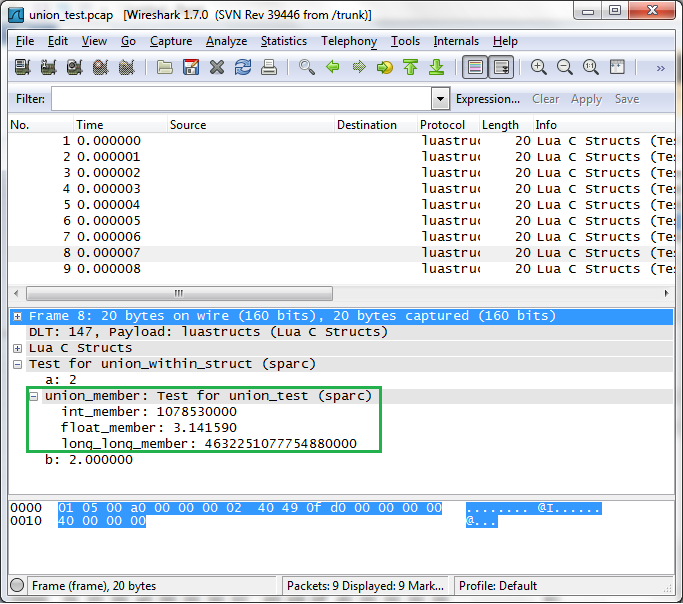
\includegraphics[width=\textwidth]{./sprints/img/wireshark_union}
	\caption{Union type support\label{fig:wsunion}}
\end{figure}

\lstset{language=C,caption={Union type},label=code:union}
\lstinputlisting[language=C]{./sprints/code/union.h}

\subsection{Display Types Wireshark Do Not Support}
%-----------------------
TODO

\subsection{Support Specifying ID of Dissectors}
%-----------------------
Specifying dissector ID has been modified from sprint 2. The dissector will 
still use the ID given in the configuration for a struct, if the struct is not 
given an ID in the configuration, then the ID for the struct will be set to 
\emph{NONE}. This is done to ensure that structs have an unique ID for their 
dissector. Structs-in-structs member do not need an ID since they are called 
from the struct' by the dissector name.

\subsection{Do Not Regenerate dissectors}
%-----------------------
TODO

\subsection{Handle Lua Reserved Keywords}
%-----------------------
Lua has a list of reserved keywords, and some of these keywords are allowed in 
the C language. The utility is able to support this under generation of Lua 
code, when an identifier is a lua keyword, an underscore(\_) is added, so the 
identifier start with ''\_''.

%-----------------------
\section{Sprint Testing}
%-----------------------
During sprint 3 the team executed a total of 9 tests were run, but no additional testingfeatures were added during the sprint. Tests executed:

\begin{itemize}
	\item TID15 - Supporting batch mode of C header and configuration files \autoref{tab:sp3TID15}
	\item TID16 - Supporting custom Lua configuration \autoref{tab:sp3TID16}
	\item TID17 - Supporting unions \autoref{tab:sp3TID17}
	\item TID18 - Supporting filter and search in wireshark \autoref{tab:sp3TID18}
	\item TID19 - Supporting WIN32, \_WIN64, \_SPARC etc \autoref{tab:sp3TID19}
	\item TID20 -  Supporting the use of flags specifying platforms to display member values correctly \autoref{tab:sp3TID20}
	\item TID21 - Supporting platforms with different endians \autoref{tab:sp3TID21}
	\item TID22 - Supporting alignments \autoref{tab:sp3TID22}
\end{itemize}

\begin{table}[!htb] \footnotesize \center
\caption{Supporting batch mode of C-headers and configuration files\label{tab:sp3TID15}}
\begin{tabular}{l l}
	\toprule
	Header & Description \\
	\midrule
	Description & Supporting batch mode of C header and configuration files \\
	Tester & Lars Solvoll Tønder \\
	Date & 28.10.2011 \\
	Result & Success\\
	\bottomrule
\end{tabular}
\end{table}

\begin{table}[!htb] \footnotesize \center
\caption{Supporting custom Lua configuration\label{tab:sp3TID16}}
\begin{tabular}{l l}
	\toprule
	Header & Description \\
	\midrule
	Description & Supporting custom LUA configuration\\
	Tester & YOUR NAME HERE \\
	Date & DATE HERE \\
	Result & TYPE THE RESULT HERE\\
	\bottomrule
\end{tabular}
\end{table}

\begin{table}[!htb] \footnotesize \center
\caption{Supporting unions\label{tab:sp3TID17}}
\begin{tabular}{l l}
	\toprule
	Header & Description \\
	\midrule
	Description & Supporting unions\\
	Tester & YOUR NAME HERE\\
	Date & DATE HERE\\
	Result & TYPE THE RESULT HERE\\
	\bottomrule
\end{tabular}
\end{table}

\begin{table}[!htb] \footnotesize \center
\caption{Supporting filter and search in wireshark\label{tab:sp3TID18}}
\begin{tabular}{l l}
	\toprule
	Header & Description \\
	\midrule
	Description & Supporting filter and search in wireshark\\
	Tester & YOUR NAME HERE \\
	Date & DATE HERE\\
	Result & TYPE THE RESULT HERE\\
	\bottomrule
\end{tabular}
\end{table}

\begin{table}[!htb] \footnotesize \center
\caption{Supporting WIN32, \_WIN64, \_sparc \label{tab:sp3TID19}}
\begin{tabular}{l l}
	\toprule
	Header & Description \\
	\midrule
	Description & Supporting WIN32, \_WIN64, \_sparc \\
	Tester & YOUR NAME HERE\\
	Date & DATE HERE\\
	Result & TYPE THE RESULT HERE\\
	\bottomrule
\end{tabular}
\end{table}

\begin{table}[!htb] \footnotesize \center
\caption{Supporting the use of flags specifying platforms to display member values correctly \label{tab:sp3TID20}}
\begin{tabular}{l l}
	\toprule
	Header & Description \\
	\midrule
	Description & Supporting the use of flags specifying platforms to display member values correctly \\
	Tester & YOUR NAME HERE\\
	Date & DATE HERE\\
	Result & TYPE THE RESULT HERE\\
	\bottomrule
\end{tabular}
\end{table}

\begin{table}[!htb] \footnotesize \center
\caption{Supporting platforms with different endian \label{tab:sp3TID21}}
\begin{tabular}{l l}
	\toprule
	Header & Description \\
	\midrule
	Description & Supporting platforms with different endian \\
	Tester & YOUR NAME HERE\\
	Date & DATE HERE\\
	Result & TYPE THE RESULT HERE\\
	\bottomrule
\end{tabular}
\end{table}

\begin{table}[!htb] \footnotesize \center
\caption{Supporting alignments \label{tab:sp3TID22}}
\begin{tabular}{l l}
	\toprule
	Header & Description \\
	\midrule
	Description & Supporting alignments \\
	Tester & YOUR NAME HERE\\
	Date & DATE HERE\\
	Result & TYPE THE RESULT HERE\\
	\bottomrule
\end{tabular}
\end{table}

\begin{table}[!htb] \footnotesize \center
\caption{Handling Lua keywords \label{tab:sp3TID22}}
\begin{tabular}{l l}
	\toprule
	Header & Description \\
	\midrule
	Description & Handling Lua keywords \\
	Tester & YOUR NAME HERE\\
	Date & DATE HERE\\
	Result & TYPE THE RESULT HERE\\
	\bottomrule
\end{tabular}
\end{table}

\subsection{Test Evaluation}

\subsubsection{Test Coverage}

%--------------------------
\section{Customer Feedback}
%--------------------------


%--------------------------
\section{Sprint Evaluation}
%--------------------------


